\subsection*{\Large Общая характеристика работы}
\fontsize{14pt}{15pt}\selectfont
\textbf{Актуальность темы.}
Визуальное моделирование --- это подход, при использовании которого программа представляется 
в виде набора графических моделей, каждая из которых описывает её с разных точек 
зрения. Благодаря наличию стандартных широко распространённых графических языков, 
визуальное моделирование повышает продуктивность труда и качество результирующего 
продукта при разработке.

Использование визуальных языков общего назначения, таких как UML, без заранее 
подготовленного набора библиотек и генераторов, делает задачу разработки 
программного обеспечения только с помощью графических языков сложной, 
в силу наличия семантического разрыва между кодом и моделями. Такие языки работают в 
тех же терминах, в которых пишется исходный код на традиционных текстовых языках 
(классы, объекты, компоненты и т.д.), поэтому, чтобы полностью специфицировать 
поведение системы и сделать возможной автоматическую генерацию, модель должна 
содержать в себе столько же информации, что и исходный код программы, но это 
противоречит самому понятию модели как некоего упрощения моделируемого объекта. 
На самом деле, визуальная модель в этом случае даже менее удобна, чем код 
программы --- визуальные символы занимают на экране больше места, чем текст. 
Если же визуальная модель будет изображать только важные аспекты 
функционирования системы, опуская излишние подробности, то её можно будет 
сохранить обозримой и полезной для человека, но это сделает её бесполезной для 
исполнителя (например, для интерпретатора или генератора исходного кода). 
Именно так, в основном, используется UML сейчас --- как средство для анализа и 
дизайна системы, а сама система специфицируется ручным кодированием на текстовых 
языках. Большинство инструментов для рисования UML-диаграмм позволяют 
сгенерировать заглушки, куда предполагается дописывать код вручную, но 
существенного выигрыша для разработчиков это не даёт. Наличие заранее подготовленных 
библиотек, шаблонов и генераторов кода может существенно улучшить ситуацию, но подобные 
технологии оказываются применимы только для той предметной области, для которой они создавались.

Существует принципиально другой подход к использованию визуального 
моделирования, называемый предметно-ориентированным моделированием. Он основан на том наблюдении, что иногда создать новый 
язык для какой-то узкой предметной области или даже для конкретной задачи и решить задачу 
на нём оказывается быстрее и эффективнее, чем решать эту задачу на языке общего назначения. 
В таком случае наличие у средств поддержки создаваемого языка знаний о предметной области 
позволяет добиться полной автоматической генерации программ про визуальным моделям.
Ряд исследований показывает, что продуктивность труда программистов при использовании 
предметно-ориентированных языков вырастает в 3-10 раз по сравнению с 
использованием языков общего назначения, поэтому такой подход представляется 
весьма перспективным.

Разумеется, создавать новый предметно-ориентированный визуальный язык и 
инструментальные средства его поддержки <<с нуля>> для каждой узкой предметной 
области или конкретной задачи было бы неоправданно трудозатратно. Поэтому 
существуют специальные средства для автоматизации этой задачи, называемые 
<<DSM-платформа>> или <<MetaCASE-средство>>. Такие средства позволяют задать 
синтаксис визуального языка, используя какой-либо формализм (как правило, 
это метамодели), и автоматически сгенерировать редактор этого языка и другие средства инструментальной 
поддержки (мы будем называть результат генерации термином <<DSM-решение>>). 
Это позволяет реализовывать технологии программирования, использующие новые предметно-ориентированные языки, за время 
порядка дней, что делает предметно-ориентированное моделирование оправданным 
даже для небольших проектов. Существуют зрелые исследовательские и промышленные 
DSM-платформы, такие как Eclipse Modeling Project, MetaEdit+ и другие; однако же, 
несмотря на значительные преимущества предметно-ориентированного 
моделирования, применяется оно довольно редко. Связано это, в частности, с 
недостатками существующих платформ и отсутствием развитой методологической 
базы для их применения. Во многих случаях для создания предметно-ориентированного 
решения требуется привлекать экспертов в создании языков, которыми зачастую 
оказываются авторы выбранной для реализации этого решения DSM-платформы, поэтому 
позволить себе это могут лишь крупные компании. Такая ситуация указывает на 
необходимость продолжения исследований в этой области с целью упростить процесс создания
предметно-ориентированных решений и снизить требования к квалификации специалистов, 
которые могли бы этим заниматься.

\textbf{Степень разработанности темы.}
Методические вопросы создания предметно-ориентированных языков хорошо проработаны в случае, если 
языки текстовые (заслуживают упоминания работы A. Van Deursen, M. Mernik), для визуальных
языков сейчас существует лишь набор слабо структурированных рекомендаций и наблюдений
(наиболее обстоятельно этим вопросом занималась исследовательская группа во главе 
со S. Kelly и J.-P. Tolvanen, заслуживают упоминания работы M. Voelter). Тем не менее, 
существует довольно много DSM-платформ, многие из которых хорошо описаны в литературе 
(MetaEdit+, Eclipse Modeling Project, Generic Modeling Environment, PSL/PSA, AToM\textsuperscript{3},
Microsoft Modeling SDK, Pounamu, DOME, MetaLanguage), анализ возможностей данных
платформ занимает значительную часть главы 2 данной работы. Подавляющее большинство 
научных работ, связанных с этими DSM-платформами, сфокусированы на технических подробностях
их реализации и обходят стороной вопросы методической поддержки, при этом часто внимание 
уделяется только самой визуализации визуального языка.

Данная работа выполнялась в рамках проекта по разработке DSM-платформы QReal, аналога
вышеперечисленных DSM-платформ, разрабатываемого на кафедре системного программирования
Санкт-Петербургского государственного университета. Эта среда разрабатывается в рамках 
деятельности научно-исследовательской группы по изучению визуального моделирования 
под руководством проф. А.Н.~Терехова с 2007 года и базируется на более чем двадцатилетнем 
опыте в разработке графических языков (технологии RTST, RTST++, REAL). Проект QReal имеет 
открытый исходный код\footnote{Страница проекта и репозиторий с исходным кодом на GitHub, URL: https://github.com/qreal/qreal}, 
разрабатывается на языке C++ с использованием библиотеки Qt силами студентов и преподавателей 
кафедры, автор данной диссертации --- один из руководителей проекта.

\textbf{Целью} диссертационной работы является уменьшение трудозатрат и требований к квалификации
при создании визуальных предметно-ориентированных языков и инструментальных средств для них (редакторов диаграмм, 
генераторов кода, средств проверки ограничений на диаграммы, интерпретаторов диаграмм)
до уровня, при котором их было бы возможно создать за время порядка часов даже без 
специальной подготовки и опыта.

Для достижения поставленной цели достаточно решить следующие \textbf{задачи}.
\begin{enumerate}
	\item Разработать методику создания предметно-ориентированных языков и инструментальных 
		средств для них, использующую визуальные языки для их спецификации.
	\item Разработать способ прототипирования визуального языка, позволяющую специфицировать его
		прямо в процессе создания на нём диаграммы.
	\item Реализовать в рамках DSM-платформы QReal простую в использовании технологию 
		создания предметно-ориентированных языков, реализующую разработанные методики.
	\item Провести апробацию технологии путём создания нескольких DSM-решений с её помощью.
\end{enumerate}

Цель и задачи диссертационной работы соответствуют области исследований паспорта специальности 
05.13.11 --- <<Математическое и программное обеспечение вычислительных машин, комплексов и компьютерных сетей>>: 
пунктам 1 (Модели, методы и алгоритмы проектирования и анализа программ и программных 
систем, их эквивалентных преобразований, верификации и тестирования) и 2 (Языки программирования 
и системы программирования, семантика программ).

\textbf{Объектом исследования} являются визуальные языки, \textbf{предметом исследования} 
являются методы их создания и технологии для разработки инструментальных средств визуальных языков.

В качестве \textbf{методологии и методов исследования} используются методы теории 
формальных языков, теории графов, методы объектно-ориентированного программирования,
эмпирические методы (методы анализа литературы и постановки эксперимента).

\textbf{Научная новизна} данной работы заключается в следующем.
\begin{enumerate}
	\item Разработана методика для создания предметно-ориентированных языков с помощью 
		графического языка метамоделирования и сопутствующих визуальных языков. Методика 
		предполагает применение предметно-ориентированного подхода <<самого к себе>>, то есть
		предметно-ориентированные языки используются для описания всей функциональности 
		разрабатываемых инструментальных средств для нового языка: редактора диаграмм, 
		генераторов текстового кода по диаграммам, интерпретаторов, средств проверки ограничений 
		на диаграммы, средств поддержки рефакторингов. Методика превосходит известные аналоги 
		по объёму функциональных возможностей инструментальных средств, которые можно 
		специфицировать с помощью визуальных языков.
	\item Предложен способ создания предметно-ориентированного языка: <<метамоделирование на лету>>. 
		Способ предполагает изменение и дополнение визуального языка прямо в процессе создания диаграммы на нём,
		без использования отдельного метаредактора. В процессе разработки языка при таком подходе
		не требуется оперировать с понятиями <<метамодель>> и <<метаредактор>>, что снижает 
		требования к квалификации пользователей. Предложенный способ является оригинальным.
	\item С использованием предложенных методик разработаны новые предметно-ориентированные языки и
		средства инструментальной поддержки для них: язык программирования роботов и среда QReal:Robots
		(также известная как TRIK Studio), средство программирования приложений для мобильных телефонов 
		QReal:Ubiq, средство разработки аппаратных систем QReal:HaSCoL.
\end{enumerate}

\textbf{Теоретическая и практическая значимость} данной работы определяется разработанными 
методами создания визуальных предметно-ориентированных языков и использованием полученных 
результатов при разработке DSM-платформы QReal, а также ряде DSM-решений, созданных с её помощью, 
самым зрелым из которых стала среда программирования роботов QReal:Robots (TRIK Studio), 
предназначенная для обучения школьников основам информатики и кибернетики с использованием робототехнических 
конструкторов ТРИК, Lego Mindstorms NXT, Lego Mindstorms EV3.

QReal создаётся как средство визуального моделирования, поддерживающее ряд широкоизвестных 
визуальных языков (UML 2.0, BPMN, блок-схемы), и одновременно как DSM-платформа, 
позволяющая быстро и без специальных знаний создавать свои собственные 
визуальные языки и DSM-решения на их основе. На данный момент среда существует 
в виде работающего прототипа. Проект поддержан грантом Санкт-Петербургского 
государственного университета 6.39.1054.2012. DSM-платформа QReal использовалась
для реализации ряда предметно-ориентированных решений, использовавшихся в 
проектах компании <<ЛАНИТ-Терком>>, связанных с разработкой информационных систем 
и систем компьютерного зрения.

Среда программирования роботов QReal:Robots (или TRIK Studio) --- на данный момент наиболее зрелая 
предметно-ориентированная технология, созданная с помощью среды QReal. 
Первый прототип среды программирования был разработан автором данной диссертации
с использованием системы QReal примерно за неделю и включал в себя визуальный 
язык из примерно 20 сущностей, редактор к нему и интерпретатор, позволяющий 
исполнить программу на компьютере, посылая команды роботу Lego Mindstorms NXT по интерфейсу 
Bluetooth. На данный момент система переименована в TRIK Studio и обладает возможностями управления роботами 
ТРИК, Lego Mindstorms NXT, Lego Mindstorms EV3 по WiFi, Bluetooth, USB, генерации программы с 
последующей загрузкой её на робот для автономного исполнения и исполнения 
программы на двухмерной модели робота на экране компьютера.

Среда QReal:Robots демонстрировалась на Открытых состязаниях Санкт-Петербурга по робототехнике 
в 2012 году и на робототехническом фестивале <<Робофест 2012>> в Москве. На данный 
момент эта среда переименована в TRIK Studio и используется как основное средство 
программирования кибернетического конструктора ТРИК, используется в нескольких робототехнических 
кружках в России и на мастер-классах по робототехнике, проводимых компанией <<Кибернетические технологии>>.

\textbf{Степень достоверности и апробация результатов} раскрывается следующим.
\begin{itemize}
	\item Некоторые результаты данной работы были представлены на второй 
		научно-технической конференции молодых специалистов <<Старт в будущее>> 
		\cite{kuzenkova2011metamodeling2}. Доклад был отмечен наградой.
	\item Результаты работы были представлены на международной конференции 
		<<8th International Conference on Evaluation of Novel Approaches to Software Engineering>> 
		(ENASE-2013)~\citescopus{kuzenkova2013qreal}.
	\item Результаты, связанные с применением разработанной технологии при 
		создании среды QReal:Robots, были доложены на VII Международной 
		научно-практической конференции <<Современные информационные технологии 
		и ИТ-образование>>~\cite{litvinov2012robots} и на конференции <<Central \& Eastern European
		Software Engineering Conference in Russia --- 2013>> (CEE-SECR'13)~\cite{terekhov2013secr}.
	\item Результаты, связанные с применением разработанной технологии для 
		разработки предметно-ориентированного языка для платформы Ubiq, были доложены 
		на международной конференции <<10th Conference of Open Innovations 
		Association FRUCT>>~\cite{bryksin2011ubiq}.
	\item Результаты, связанные с использованием предлагаемой технологии неоднократно 
		представлялись сообществу в виде научных публикаций~\cite{kuzenkova2011qreal, litvinov2013robots,
		terekhov2013qreal, osechkina2010gestures, terekhov2009architecture}
		и докладов на конференциях соавторами работ~\cite{terekhov2013robots, kuzenkova2013refactoring,
		osechkina2012multistroke, bryksin2011qreal, kuzenkova2011metamodeling, bryksin2011robots}.
\end{itemize}

\textbf{Публикации}. Результаты диссертации отражены в пяти научных работах и одиннадцати тезисах докладов, 
основные результаты изложены в журналах, входящих в перечень ведущих рецензируемых научных 
журналов и изданий, в которых должны быть опубликованы основные научные результаты диссертаций 
на соискание ученых степеней доктора и кандидата наук, утвержденный решением Президиума 
Высшей аттестационной комиссии Минобрнауки России (\citevak{litvinov2013robots, kuzenkova2011qreal, terekhov2013qreal}),
\cite{terekhov2009architecture, osechkina2010gestures} --- в журнале, входящем в РИНЦ, и 
в одиннадцати тезисах докладов на конференциях (под авторством или в соавторстве с автором 
диссертации). Работы в сборниках из перечня ВАК \cite{kuzenkova2011qreal} и \cite{terekhov2013qreal}
написаны в соавторстве. В работе \cite{kuzenkova2011qreal} автору данной диссертации 
принадлежит проектирование и разработка средств метамоделирования, Т.А. Брыксину --- архитектура и реализация основных
компонент платформы, А.С. Кузенковой --- реализация некоторых частей метаредактора, А.О. Дерипаска
--- реализация редактора форм фигур системы QReal, А.В. Подкопаеву --- реализация средств задания правил генерации кода,
К.С. Тарану --- реализация средств эволюции визуальных языков. В работе \cite{terekhov2013qreal}
автору данной диссертации принадлежит идея и реализация средств метамоделирования, А.Н. Терехову 
принадлежит постановка задачи, Т.А. Брыксину --- разработка архитектуры и реализация основных модулей платформы QReal.

\textbf{Личный вклад автора.} Результаты, представленные в диссертационной работе, получены 
соискателем либо самостоятельно, либо при его непосредственном участии.

Проект QReal в силу своей трудоёмкости разрабатывается большой группой студентов, аспирантов
и преподавателей кафедры системного программирования СПбГУ, соискатель претендует лишь на
результаты, явно перечисленные в списке положений, выносимых на защиту.

Хочется отметить вклад в проект QReal студентов, работавших над проектом QReal под руководством 
соискателя: Абрамова Ивана Александровича, Дерипаска Анны Олеговны, Гудошниковой Анны Андреевны, 
Жуковой Беллы Юрьевны, Заболотных Елены Петровны, Занько Софьи Владимировны, Иванова Всеволода Юрьевича, 
Кузенковой Анастасии Сергеевны, Кузнецовой Марьи Юрьевны, Курбанова Рауфа Эльшад оглы, 
Назаренко Владимира Владимировича, Нефёдова Ефима Андреевича, Никольского Кирилла Андреевича, 
Осечкиной Марии Сергеевны, Птахиной Алины Ивановны, Пышновой Александры Витальевны, 
Савина Никиты Сергеевича, Соковиковой Натальи Алексеевны, Такун Евгении Игоревны, 
Тихоновой Марии Валерьевны, всех студентов, работавших под руководством Брыксина Тимофея Александровича, 
а также вклад Дмитрия Мордвинова и Ирины Брюхановой.

\textbf{Структура и объём работы.} Диссертация состоит из введения, четырёх глав, заключения, 
списка сокращений и условных обозначений, списка литературы (120 наименований) и двух приложений. Объем основной 
части работы --- 127 страниц с 19 рисунками, 2 таблицами и 3 листингами.

\subsection*{\Large Положения, выносимые на защиту}
\begin{enumerate}
	\item Разработана методика для создания предметно-ориентированных языков с помощью 
		графического языка метамоделирования и сопутствующих визуальных языков.
	\item Предложен новый способ метамоделирования: <<метамоделирование на лету>>, позволяющий
		создавать визуальный язык в процессе его использования.
	\item Предложенные методики реализованы в виде технологии на базе системы QReal.
	\item Проведена апробация разработанных методик и технологии при создании редактора, 
		генератора, средств проверки ограничений среды QReal:Robots и других предметно-ориентированных 
		решений.
\end{enumerate}

\subsection*{\Large Содержание работы}
Во \textbf{введении} обосновывается актуальность исследований, проводимых в рамках 
данной диссертационной работы, формулируется цель работы, научная новизна и практическая 
значимость, приводятся сведения об апробации работы.

В \textbf{Главе 1} приводятся основные понятия, используемые в 
предметно-ориентированном визуальном моделировании. Обсуждается структура 
визуального языка: синтаксис (абстрактный, конкретный и синтаксис сериализации), 
уровни абстракции (предметная область, модель, метамодель, метаметамодель), вводится 
классификация формальных языков по важным для дальнейшего изложения свойствам.

По форме представления информации языки делятся на следующие группы: \textit{текстовые} языки 
--- используют в основном текст для представления информации, \textit{графические} или 
\textit{визуальные} языки, использующие визуальные символы, и \textit{текстографические} языки,
активно использующие и текст, и графику для представления программы. Графические языки, в свою очередь, 
делятся на графовые (в которых диаграмма представляет собой помеченный мультиграф, либо сводится к нему)
и неграфовые (не сводящиеся к помеченному мультиграфу).

По используемой модели вычислений языки делятся на \textit{статические} (задающие структуру разрабатываемой системы) \
и \textit{динамические} (описывающие поведение), которые, в свою очередь, делятся на языки, 
модель вычислений которых основана на сетях Петри (с простыми токенами --- ориентированные на поток управления,
или с токенами, содержащими в себе существенную информацию --- ориентированные на поток данных),
и языки, в основе которых лежат диаграммы конечных автоматов.

\textbf{Глава 2} содержит обзор существующих подходов к созданию DSM-решений. 
Рассматриваются существующие методологии разработки предметно-ориентированных языков,
обсуждаются возможности, достоинства и недостатки существующих DSM-платформ, 
включая зрелые системы и академические разработки. Результаты анализа существующих 
DSM-платформ сведены в таблицу \ref{tab:existingPlatformsMain}.

\begin{table}[!ht]
\begin{small}
	\begin{longtabu} {| X[1 l p] | X[1 l p] | X[1 l p] | X[1 l p] |X[1 l p] |}
		\caption{Основные возможности существующих DSM-платформ} \\
		\tabucline-
		 Название                    & Метаязык                        & Метаредактор                                            & Конкретный синтаксис                                     & Ограничения                                    \\
		\tabucline-
		\everyrow{\tabucline-}
		MetaEdit+                    & GOPPRR                          & Визуальный или диалоговые окна                          & Визуально                                                & Только средствами метаязыка                    \\
		Eclipse Modeling Project     & Ecore (аналог MOF)              & Визуальный, текстовый, импорт метамодели                & Визуально или вручную поверх библиотек                   & Текстовые (OCL)                                \\
		Generic Modeling Environment & Свой, довольно развитый         & Визуальный                                              & Настройкой существующих фигур                            & Текстовые (OCL)                                \\
		PSL/PSA                      & Сущность-связь                  & Текстовый                                               & Нет                                                      & Нет                                            \\
		AToM3                        & Сущность-связь                  & Визуальный                                              & Визуально                                                & Вручную, на Python                             \\
		Microsoft Modeling SDK       & Свой (диаграммы классов)        & Визуальный                                              & Настройкой существующих фигур или кодированием на C\#    & Вручную поверх библиотеки                      \\
		Pounamu                      & Сущность-связь                  & Визуальный                                              & Визуально                                                & Визуальным языком общего назначения или Java   \\
		DOME                         & Свой (DSTL), довольно развитый  & Визуальный                                              & Настройкой существующих фигур или кодированием на Alter  & Вручную, на Alter                              \\
		MetaLanguage                 & Сущность-связь                  & Визуальный                                              & Неизвестно                                               & Да                                             
		\label{tab:existingPlatformsMain}
	\end{longtabu}
\end{small}
\end{table}

Делаются выводы о том, что все существующие среды не автоматизируют весь жизненный цикл
создания предметно-ориентированного решения, особенно его начальные этапы --- если автор DSM-решения уже 
<<знает, что писать>> (то есть имеет в голове ясное представление о предметной области 
и даже метамодель создаваемого языка), то к его услугам множество существующих инструментов. 
Но если требуется вести разработку предметно-ориентированного решения <<с нуля>> (начиная 
с оценки осуществимости и анализа предметной области), очень многое придётся делать 
без какой-либо инструментальной поддержки и, как правило, без руководства к действию.
Таким образом, явно имеется пробел в существующих исследованиях, который данная работа
призвана помочь заполнить.

\textbf{Глава 3} содержит описание предлагаемого подхода к разработке 
DSM-решений: приводятся этапы жизненного цикла DSM-решения, обсуждается 
возможная степень автоматизации каждого этапа, формулируются требования на 
средства автоматизации, приводится описание предлагаемой технологии. Предлагается
два варианта методологии разработки --- <<Классическая>> методология и методология <<Метамоделирования
на лету>>, которая является вариантом классической и служит для упрощения первых этапов
жизненного цикла DSM-решения. Схематически <<Классическая>> методология изображена на рисунке
\ref{classicMethodology}.

\begin{figure} [ht]
	\begin{center}
		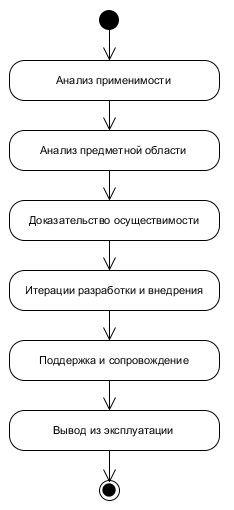
\includegraphics[width=0.25\textwidth]{part3/classicMethodology.png}
		\caption{<<Классическая>> методология разработки визуального предметно-ориентированного языка.}
		\label{classicMethodology}
	\end{center}
\end{figure}

Фаза разработки и внедрения состоит из нескольких итераций, порядок действий для каждой 
из которых представлен на рисунке~\ref{classicMethodologyIteration}. 

\begin{figure} [ht]
	\begin{center}
		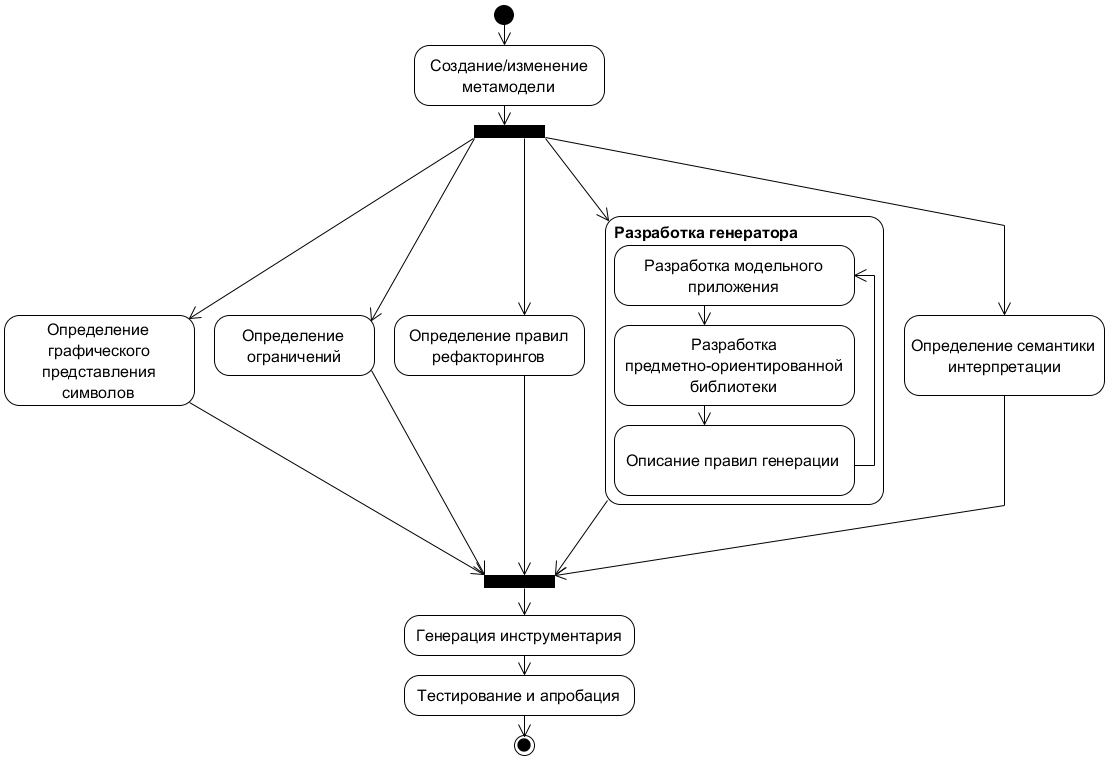
\includegraphics[width=0.9\textwidth]{part3/classicMethodologyIteration.png}
		\caption{Итерация проектирования и разработки языка.}
		\label{classicMethodologyIteration}
	\end{center}
\end{figure}

Такая методология называется классической, поскольку примерно такой схемы придерживается
большинство существующих DSM-платформ и большинство авторов, описывающих процесс создания
предметно-ориентированных языков и дающих рекомендации по этому процессу. Вклад данного 
исследования состоит в структуризации этапов жизненного цикла, описании действий на 
каждом этапе жизненного цикла и предложения технологии автоматизации каждого этапа.
Основная идея, предлагаемая здесь --- использование визуальных языков на каждом
этапе жизненного цикла, вплоть до описания генераторов.

С методологической точки зрения научную новизну имеет предлагаемый здесь подход 
<<Метамоделирования на лету>>. Ключевой принцип данной методологии состоит в том, 
что создание визуального языка проходит непосредственно в процессе рисования диаграммы, 
без использования метаредактора.

Основной этап предлагаемой методологии --- прототипирование языка --- начинается сразу 
после этапа анализа применимости. Разработчик языка и будущий пользователь работают 
за одним рабочим местом. При запуске DSM-платформы они видят канву для рисования и 
пустую палитру. Пользователь объясняет, что он примерно хотел бы нарисовать, разработчик 
языка добавляет на палитру новые элементы, определяет для них графическое представление, 
пользователь рисует. Пользователь может сказать, что такой-то элемент должен содержать 
такую-то дополнительную информацию, тогда разработчик добавляет элементу новое свойство, 
задаёт его тип и значение по умолчанию, и пользователь продолжает рисовать диаграмму, 
используя новое свойство. Через некоторое время пользователь может сам добавлять и 
редактировать типы элементов, и работа полностью передаётся ему, разработчик языка 
лишь следит за процессом и консультирует при необходимости пользователя. Работа заканчивается, 
когда модельное приложение полностью нарисовано, после чего текущая интерпретируемая 
метамодель сохраняется в виде, пригодном для дальнейшего редактирования в метаредакторе. 
После этой фазы идут итерации <<классической>> методологии по доработке созданного 
прототипа, дополнению его ограничениями, рефакторингами, интерпретатором и генератором, 
подготовки инсталляционного пакета, развертывания и сбора обратной связи. На этих этапах 
пользователи, как и в <<классической>> модели, непосредственно в разработке не участвуют, 
поскольку этапы гораздо более продолжительны во времени и прямо при пользователе выполнены 
быть не могут.

Модель жизненного цикла языка, использующая <<метамоделирование на лету>>, представлена 
на рисунке~\ref{metamodelingOnFly}.

\begin{figure} [ht]
	\begin{center}
		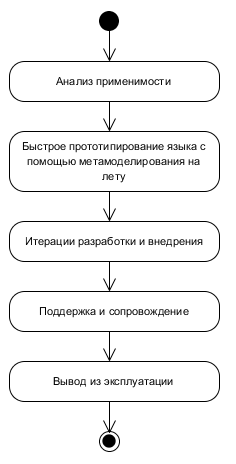
\includegraphics[width=0.25\textwidth]{part3/metamodelingOnFly.png}
		\caption{Методология <<метамоделирования на лету>>.}
		\label{metamodelingOnFly}
	\end{center}
\end{figure}

В \textbf{Главе 4} анализируются результаты реализации инструментальных средств поддержки предлагаемой 
технологии в проекте QReal. Описываются возможности системы QReal, связанные с поддержкой 
техник метамоделирования, включая метамоделирование на лету, принятые архитектурные 
решения.

\textbf{Приложение A} содержит примеры применения результатов, описанных в данной 
диссертации, для разработки DSM-решений. Описывается среда QReal:Robots, то, какие 
преимущества были получены от использования DSM-платформы QReal при её разработке, 
то, чем QReal помочь не смог, и почему. Также приводится описание среды разработки 
сервисов для мобильных телефонов QReal:Ubiq и среды разработки аппаратуры QReal:HaSCoL, 
описываются их визуальные языки, достоинства и недостатки принятых при их создании подходов.

В \textbf{Приложении B} описывается визуальный метаязык системы QReal.

В \textbf{заключении} приведены итоги выполненного исследования, рекомендации и перспективы дальнейшего развития.
